
\subsubsection{Displacement simulation}\label{sec:DisplacementSimulation}
The effect of data qubit displacement considered in the proposal \cite{OGorman2016}, and using a simulation of the logical surface code operations, a code threshold of $R=\SI{6.1}{\nano\metre}$ was derived. We will now look more closely at the magnitude and character of errors that happen from displacements close to this threshold. 

We ran 800 simulations for even parity with no bit-flips, and 800 for odd parity with a randomly chosen bit-flip. The full dynamics of the interaction Hamiltonian derived in section \ref{sec:dipole-dipole} was simulated for each run, with randomly generated qubit displacements within the pillbox region illustrated in fig.\@ \ref{fig:pillbox} for $R = \SI{6}{\nano\metre}$, within the code threshold. Finally, to ensure the full scheme as proposed was being implemented, randomly chosen twirling operations were added.

The 1600 simulation runs consumed 96 computer-hours, yielding the histogram in fig.\@ \ref{fig:DisplacementHistogram}. Two peaks are observed, with no significant deviation from $\pi$/$2\pi$, but the standard deviations of \num{0.265+-0.001} yield rotations from the mean of up to $\tfrac{\pi}{4}$, corresponding to a \SI{14.6}{\percent} error rate for the worst case simulated.

Projecting onto the $x$-axis, however, we find that the average measurement success probability is $\mathrm{P(\ket{+}) = \SI{99.9}{\percent}}$ for even parity and $\mathrm{P(\ket{-}) = \SI{96.7}{\percent}}$ for odd parity, which for low bit-flip rates is well within the \SI{98.9}{\percent} threshold for the surface code, and the standard deviation in phase represents \SI{4.2}{\percent} of $2\pi$, less than the \SI{4.4}{\percent} phase jitter the proposal \cite{OGorman2016} used to derive the results from the logical surface code simulation.

Thus we can conclude that, though the interaction strength has a high $\tfrac{1}{r^3}$ dependence, the parity measurement appears surprisingly tolerant to qubit displacement. Additionally, with the phase variance at the code threshold for qubit displacement being within the phase jitter parameter implemented in the proposal's logical simulations, the results of their simulation likely hold true for any qubit implantation technique with a precision within the $R=\SI{6.1}{\nano\metre}$.


\begin{figure}
	\centering
	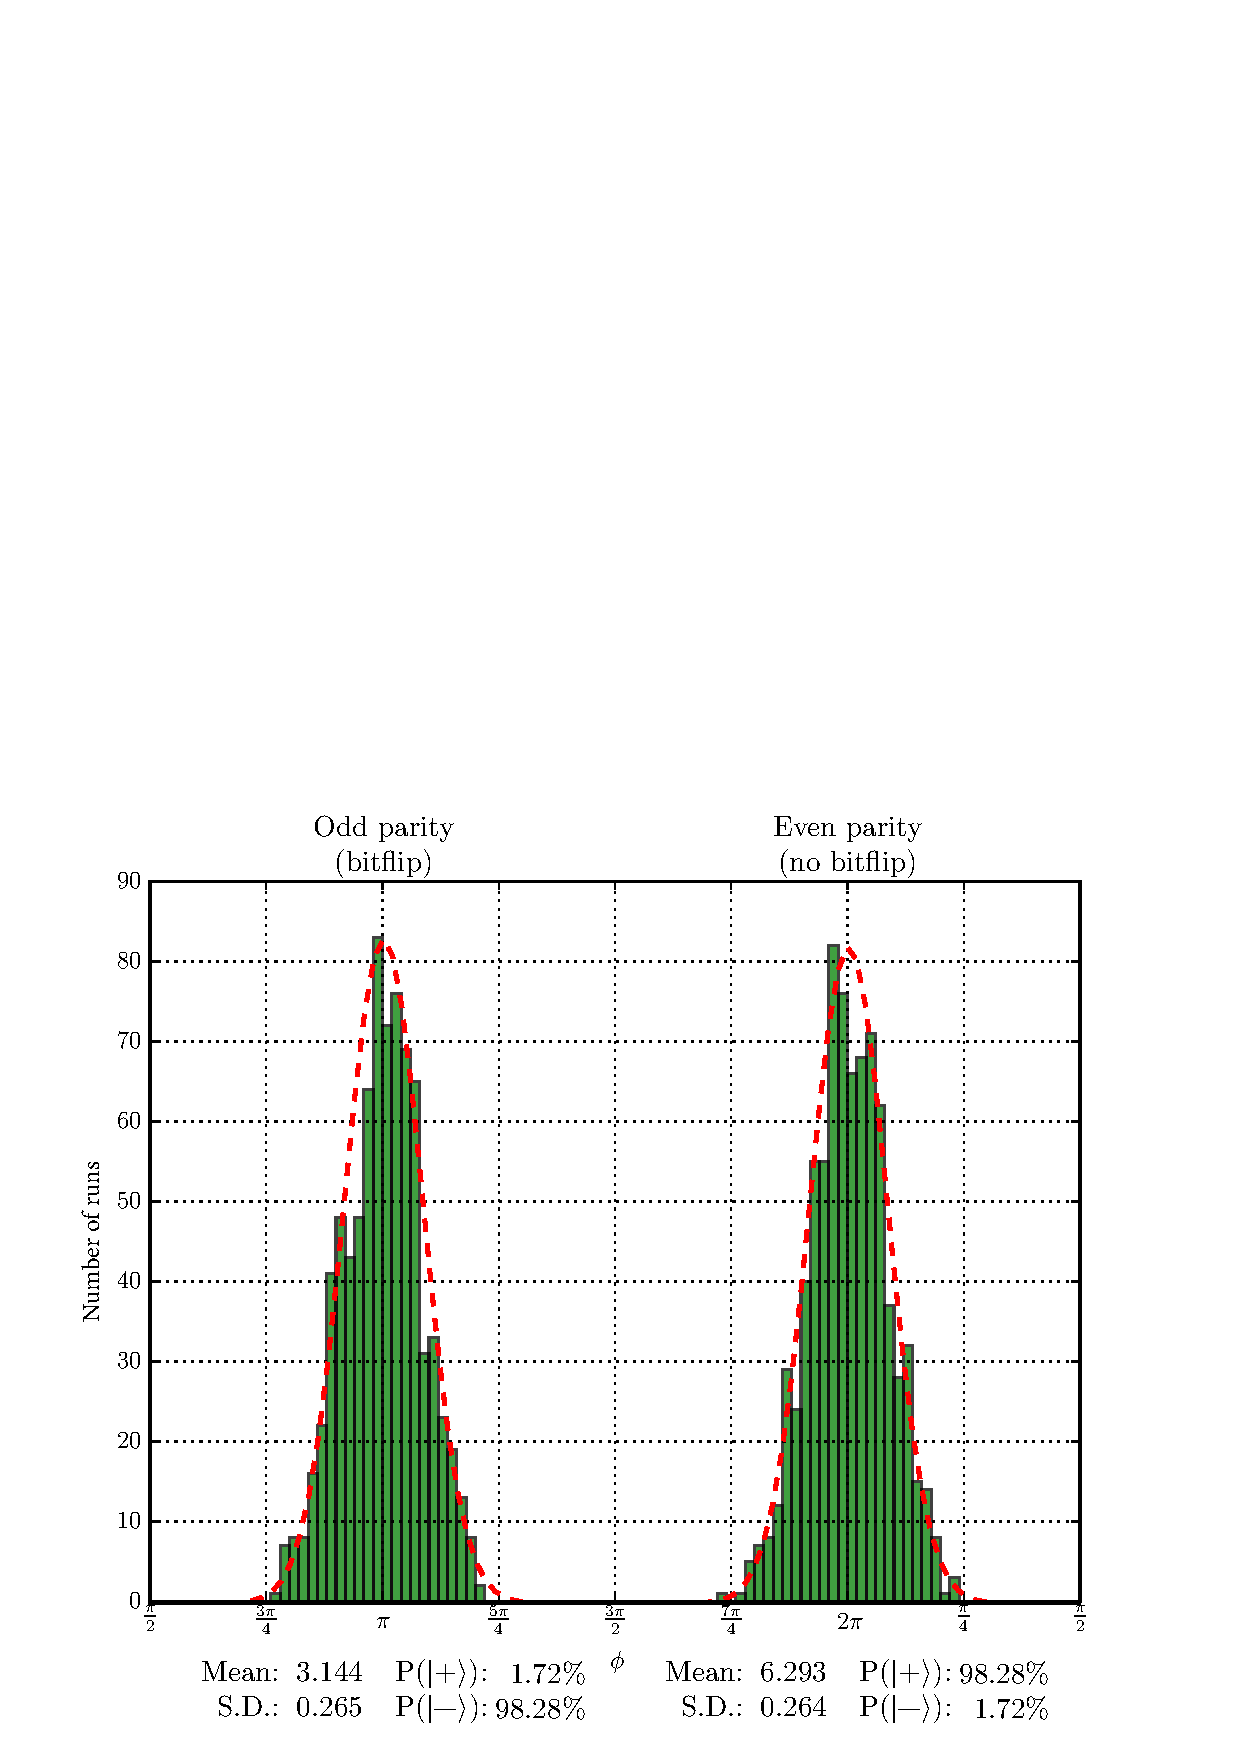
\includegraphics[width=\columnwidth]{../Figures/Displacement_Histogram.pdf}	
	\caption{Phase errors over 25 runs as a result of randomly generated data qubit displacements within a pillbox of half-height \SI{3}{\nano\metre} and radius \SI{6}{\nano\metre}. These values are a threshold for the proposed scheme.}
	\label{fig:DisplacementHistogram}
\end{figure}